\section{Mac OS}
\subsection{Histoire}
C'est en 1976 que le Apple Computer 1, rétroactivement appelé Apple I, est mis
en vente par la \textit{Apple Computer Company} - maintenant appelée
\textit{Apple Inc.} et créée le 1er avril 1976. \\
C'est alors l'un des tout premiers micro-ordinateurs individuels. \\

Alors que Steve Jobs en fait la publicité, il est construit à la main par Steve
Wozniak qui en créa le langage assembleur en BASIC (\textit{en ne passant que
par de l'hexadécimal}) afin de pouvoir programmer des jeux et y jouer. \\
En effet, l'Apple I était principalement fait pour jouer. \\

L'Apple II sort un an plus tard, le système est le même et donne la possibilité
à tous de créer des programmes utilisant les toutes dernières nouveautés: la
couleur et le son. Cependant, il y avait un gros inconvénient: les utilisateurs
devaient stocker leurs données sur des cassettes, cette méthode étant, on s'en
doute, très lente, incommode et peu fiable.

\begin{figure}[!htb] \minipage{0.45\textwidth}
  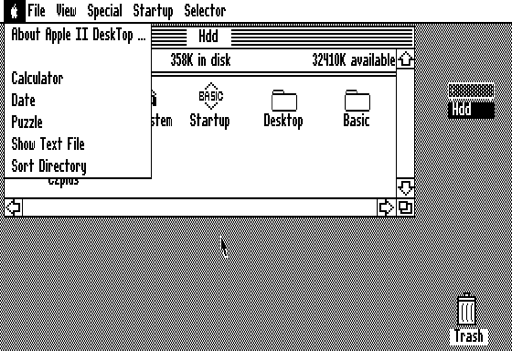
\includegraphics[width=\linewidth]{textures/images/mac/historic/apple2.png}
  \caption{Apple II Desktop}\label{fig:Apple II Desktop}
	\endminipage\hfill \minipage{0.45\textwidth}
  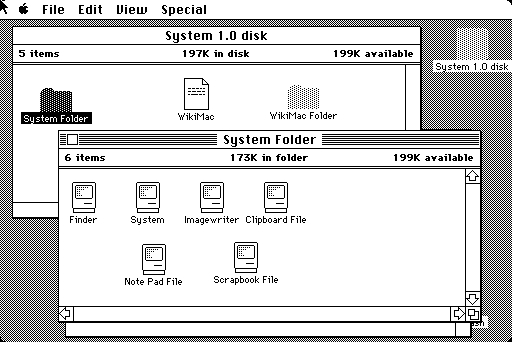
\includegraphics[width=\linewidth]{textures/images/mac/historic/system1.png}
  \caption{System 1}\label{fig:System 1}
	\endminipage
\end{figure}

Pour régler ce problème, le DOS 3.1 (\textit{Disk Operating System}) est rendu
disponible en 1978 et sera mis à jour jusqu'en 1980 avec la version 3.3. \\
Le système d'exploitation permet d’utiliser des disques durs et des disquettes
comme périphériques de stockage. \\

Comme le dit si bien l'adage : "\textit{Jamais deux sans trois.}". La même
année, sort l'Apple III accompagné du SOS (\textit{Sophisticated Operating
System}). \\ C'est le premier OS pour micro-ordinateur à utiliser le
concept de drivers qui aident l’ordinateur à communiquer avec les périphériques
(\textit{disques durs, clavier, écran}), ce qui lui offrit une flexibilité à
utiliser de nouvelles technologies.

\newpage

Une mise à jour du système d'exploitation des Apple II arrive en 1983, ProDOS
(\textit{Professional Disk Operating System}) utilise la même structure de
fichiers que SOS ce qui permet d’utiliser un même disque sur un Apple II et sur
un Apple III, ainsi que de partager des fichiers entre ces ordinateurs. ProDOS
ajoute aussi la compatibilité avec un plus grand nombre de disquettes et
disques durs et augmente le volume maximum de 400 kb à 32 Mb. \\

La même année sort le Lisa avec le Lisa OS qui prend en charge le multitâche et
la protection de mémoire (\textit{droit d’accès à la mémoire non allouée}). \\
De ce fait, le système de fichiers s’améliore encore et devient plus pratique
pour les disques durs à « grande capacité ». \\

Après le Lisa, vient le Macintosh avec le System 1. Les premiers Macintosh ont
utilisé des versions successives du \textit{System} numérotées de 1 à 7. C’est
à partir de la version 7.6 qu’il prend le nom de \textit{Mac OS}. La version
actuelle étant la dixième version majeure ainsi que la version UNIX du système,
son nom est devenu Mac OS X (\textit{Mac OS Ten}). \\

En effet, c'est depuis 1999 et le premier iMac que le système d'exploitation
des ordinateurs Apple est Mac OS X. Il a évolué de la version 10.0
(\textit{Cheetah}) à la version actuelle 10.11 (\textit{El Capitan}). \\

Mac OS X est la fusion entre Mac OS et NeXTSTEP (le système d’exploitation
orienté objet de \textit{NeXT}, l’entreprise fondée par Steve Jobs après son
départ en 1985). NeXTSTEP était un UNIX-like vu que basé sur un noyau Mach et
sur l’implémentation BSD d’UNIX.  \\

Depuis la version 10.5 (en 2007), le système d’exploitation possède la
certification UNIX.

\begin{figure}[!htb]
	\minipage{0.45\textwidth}
  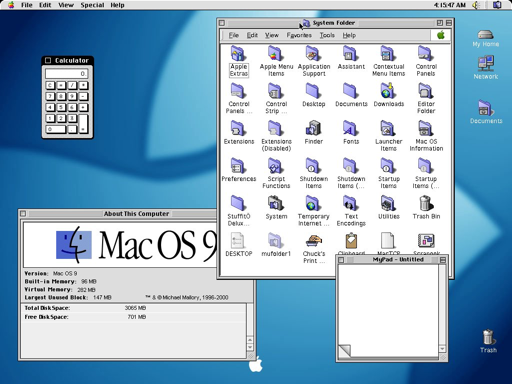
\includegraphics[width=\linewidth]{textures/images/mac/historic/macos9.png}
  \caption{Mac OS 9}\label{fig:OS 9}
	\endminipage\hfill
	\minipage{0.5\textwidth}
  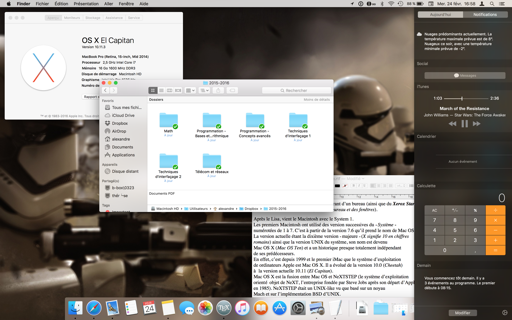
\includegraphics[width=\linewidth]{textures/images/mac/historic/macosx11.png}
  \caption{Mac OS X 10.11}\label{fig:OS X}
	\endminipage
\end{figure}

\subsection{Dérivés}

Même si elle n’est pas très connue, Apple propose une version pour serveur de
son système d’exploitation pour ordinateurs. \textit{Mac OS X Server} est rendu
disponible en tant que mise à jour téléchargeable et prend la forme d’une
simple application. Elle permet de gérer facilement des ordinateurs,
calendriers, fichiers, sauvegardes, etc. \\

Apple possède encore trois autres systèmes d’exploitation - iOS, watchOS et
tvOS basés sur Mac OS X. \\ Comme leur nom l’indique, watchOS est le système de
l’Apple Watch et tvOS est celui de l’Apple TV. iOS est celui des
\textit{iDevices} c’est-à-dire les iPhone, iPad et iPod Touch, son nom vient de
iPhoneOS devenu iOS en 2010, lors de la sortie du premier iPad. \\

Leur base étant la même, certaines applications n’ont pas besoin d’être
entièrement réécrites pour être portées sur une autre plateforme
(\textit{celles d'Apple tout du moins}). Par exemple, l’app Photos sur Mac OS X
n’a pas nécessité beaucoup de changements pour être portée sur iOS. \\

De plus, certaines fonctionnalités comme les fenêtres peuvent être affichées
sur des iPad en activant certains paramètres internes cachés d’iOS. \\

Ces deux OS : Mac OS X et iOS partageant de plus en plus de fonctions, ce
seront bientôt deux systèmes ayant les mêmes fonctionnalités adaptées à leur OS
(\textit{p. ex. écran tactile pour les iDevices}). En effet, pour l’instant il
n’est pas question de fusion, mais plutôt de convergence entre ces deux OS.

  \begin{figure}[!h]
    \center
    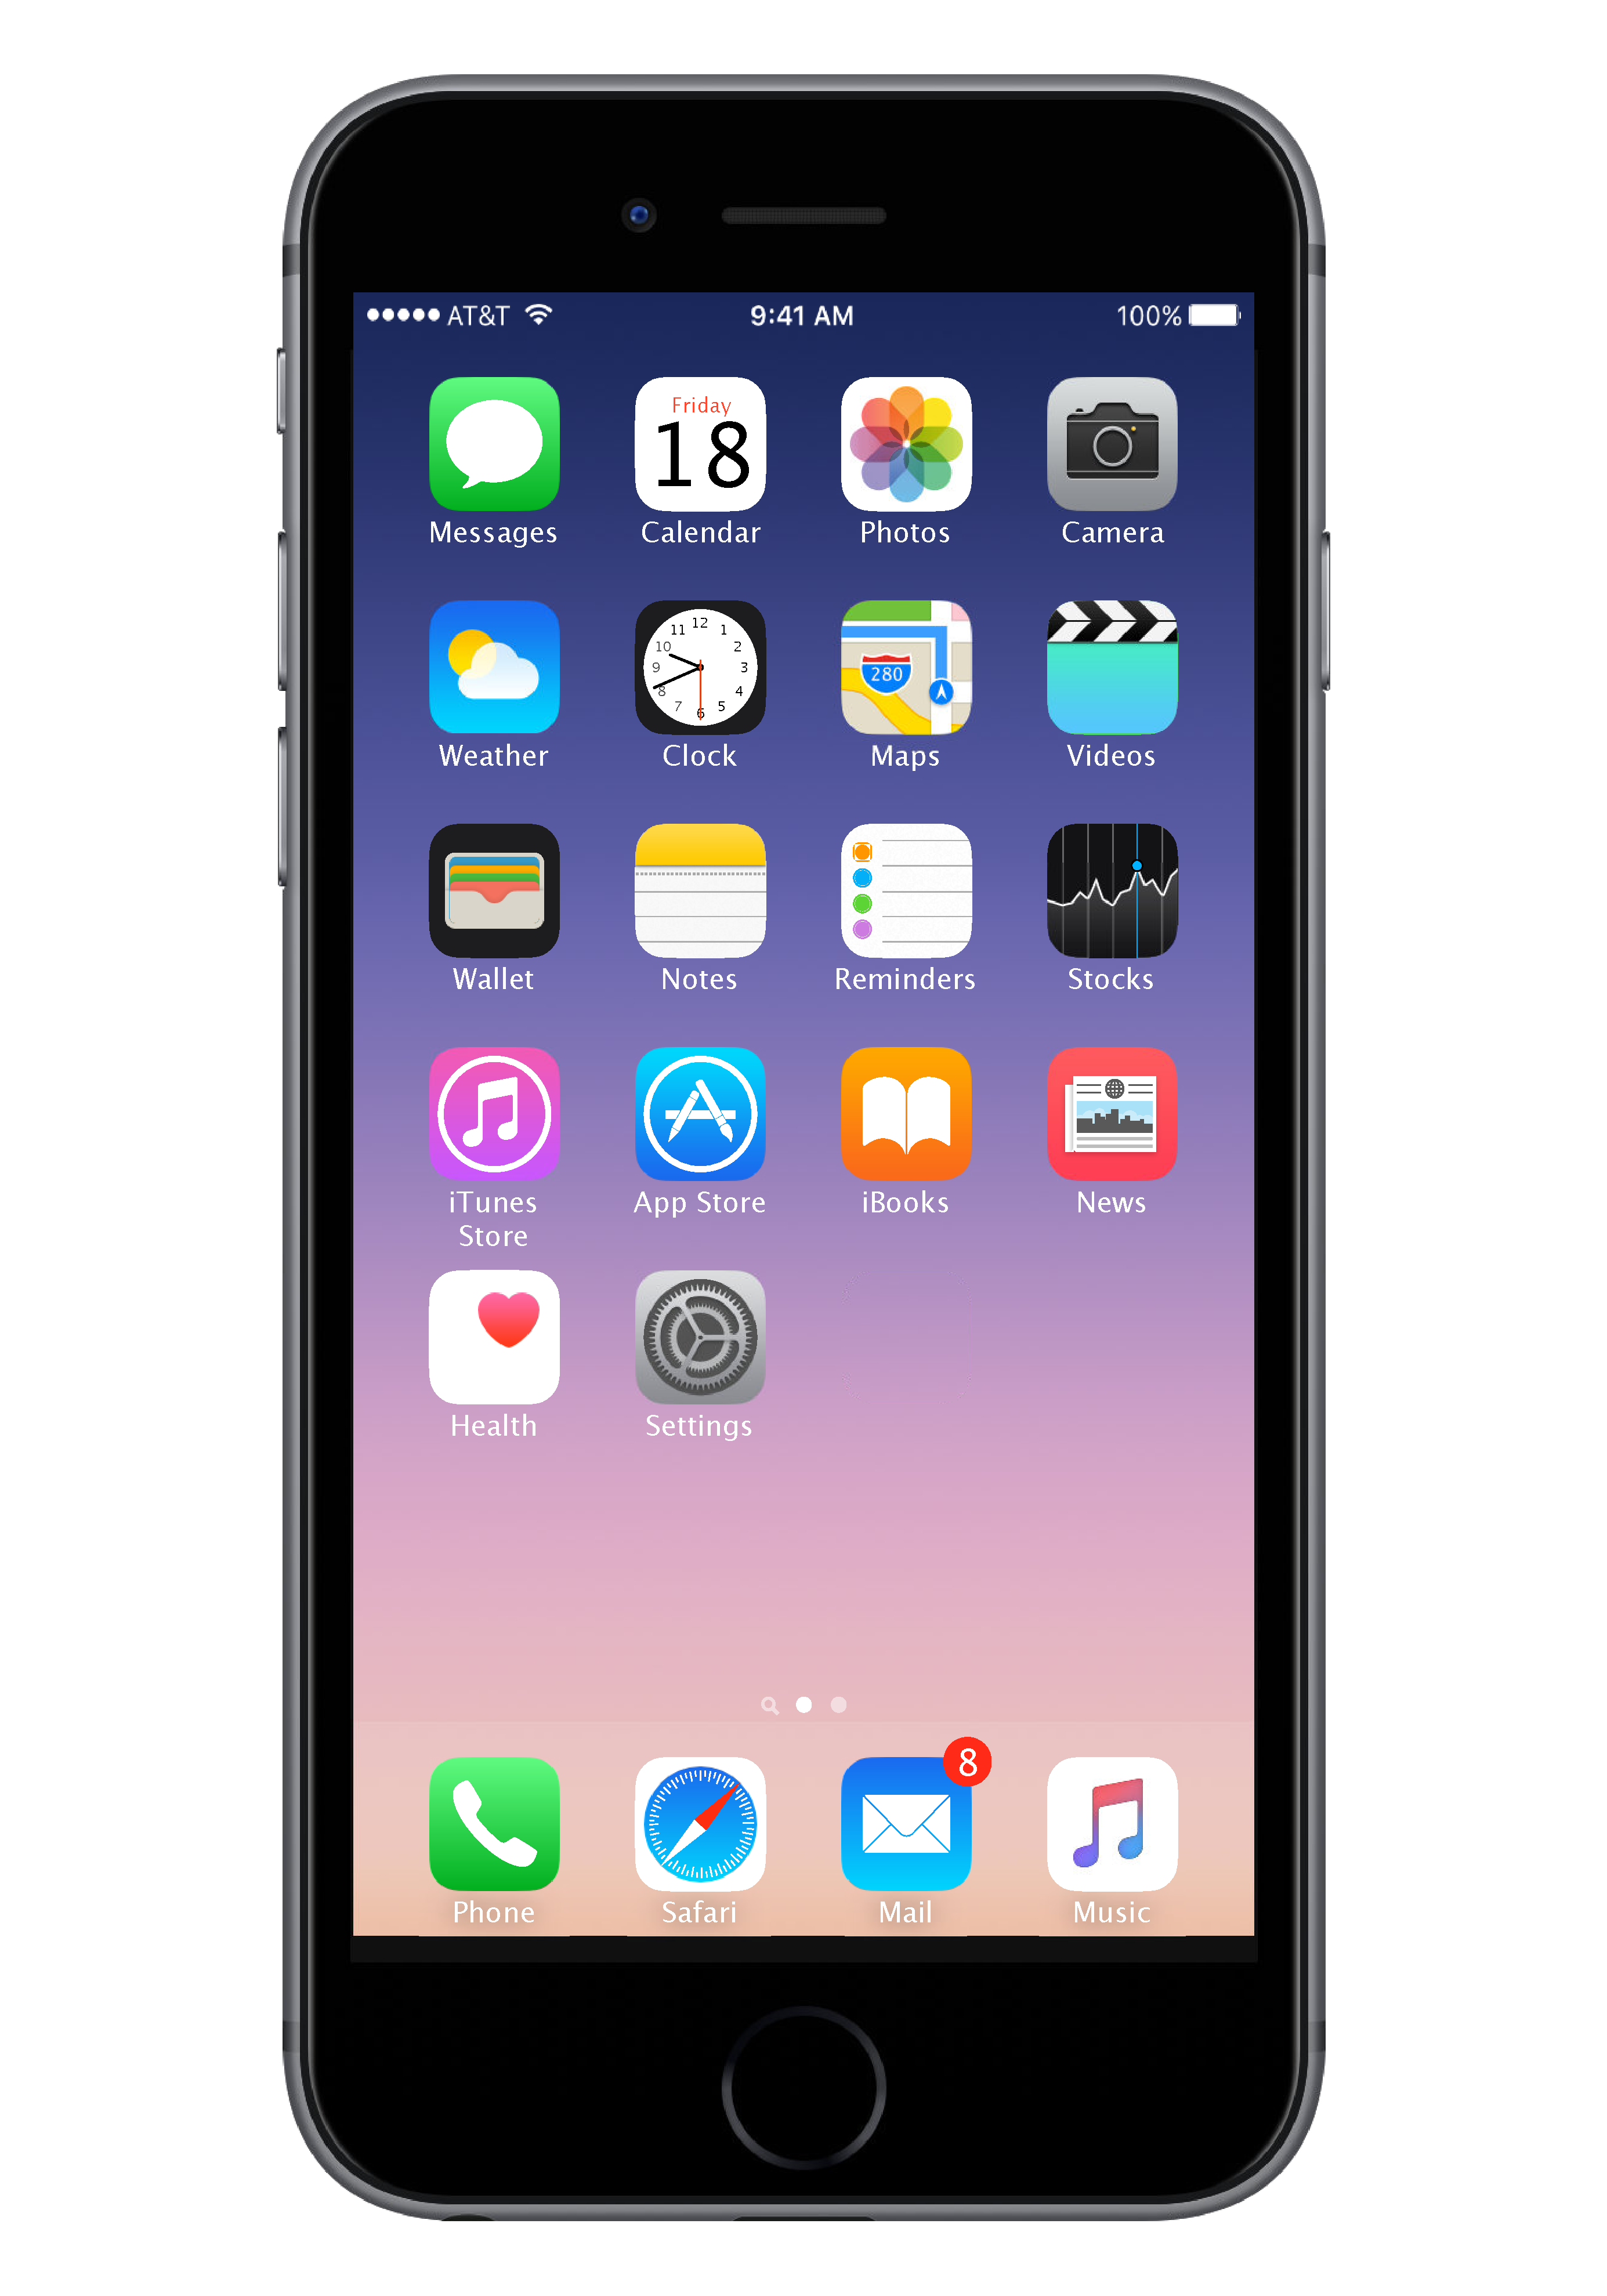
\includegraphics[scale=0.08]
    {textures/images/mac/historic/iOS.pdf}
    \caption{Système d'exploitation iOS}
  \end{figure}

\newpage

\subsection{Popularité}
Les avis à l’encontre de Mac OS X sont assez partagés. \\

Par exemple, les détracteurs pointent du doigt le prix fort élevé à l’achat
ainsi que la presque impossibilité de mise à jour matérielle des macs. \\
Par contre, ces personnes sont souvent des personnes n’ayant jamais utilisé de
Mac. Ils ont alors une vision biaisée leur faisant croire que rien n’est gratuit,
ainsi des fonctionnalités comme le \textit{couper-coller} seraient payantes, ou
bien que l’on ne peut pas faire autant de choses que sur d’autres systèmes comme
Windows. \\

Les partisans mettent par contre en avant la stabilité, la sécurité, la fiabilité
et la vitesse de l’OS. \\
Depuis des années, la facilité d’utilisation est une des forces des systèmes d’Apple,
ainsi que sa base UNIX qui offre la puissance de la ligne de commande au système. \\

Ce n’est un secret pour personne, l’augmentation des parts de marché des Macs
est principalement due à la popularité des iPods, puis principalement des iPhones
et des iPads. \\
Un point positif pour toute personne possédant un appareil Apple: les systèmes
étant proches, passer de l’un à un l’autre ne sera pas dépaysant. De plus, avoir
un ou des appareils mobiles et un mac crée un écosystème permettant de gagner du
temps ainsi que des fonctionnalités. \\

Par défaut, OS X possède de nombreuses fonctionnalités et applications
préinstallées. \\
Mais il en existe d’autres disponibles gratuitement comme \textit{Xcode},
l’IDE d’Apple nécessaire pour créer des applications iOS et qui donne accès à
des outils en ligne de commande comme un compilateur C, et \textit{iWork},
la suite bureautique d’Apple disponible aussi sur iOS et au travers de
n’importe quel navigateur web. \\

\clearpage

\subsection{Fonctionnalités}
Pour commencer, Apple a un avantage sur ses concurrents: l'entreprise ne
s'occupe pas seulement du système d'exploitation, mais aussi des ordinateurs
qui l'utilisent: ils sont donc pensés pour fonctionner en adéquation. Grâce à
cela, Apple peut sortir des sentiers battus et exploiter de nouvelles
technologies tandis que les autres constructeurs doivent attendre que l'OS dont
ils dépendent prenne en considération l'utilité de telle ou telle nouveauté. \\

Par exemple, l'utilisation d'un trackpad multitouch permettant l'utilisation de
gestes tactiles sur ordinateur existe depuis des années sur Mac, et arrive
maintenant chez la concurrence. On peut aussi parler du \textit{Thunderbolt} qui
n'est utilisé que par Apple et qui peut connecter jusqu'à 6 périphériques avec
un débit de 10 Gbit/s dans les deux sens. Son utilisation pourrait se démocratiser
avec le changement de connecteur qui passerait du Mini DisplayPort à l'USB-C et
avec le débit qui doublerait. \\

De plus, grâce au fait qu'Apple développe les systèmes d'exploitation et les
appareils qui les utilisent, un utilisateur d'iPhone ne sera pas dépaysé lors
de l'utilisation d'un Mac, et vice-versa. \\
Il est à noter qu'avec la sortie du \textit{Surface Book} de Microsoft,
Apple n'est plus la seule entreprise à proposer des ordinateurs créés en
parallèle de leur système d'exploitation. \\ Cela pourrait donner un avantage
certain à Microsoft par rapport à ses « \textit{concurrents} » sur Windows. \\

Du côté logiciel, il existe certaines fonctionnalités exclusives à Mac OS X:
\\

\begin{itemize}
\item \textbf{Quick Look} : activé avec un geste multitouch ou la barre d'espace,
permet de montrer un aperçu du fichier/dossier sélectionné sans avoir à
l'ouvrir. Sur un mot, il en donne la définition et/ou la traduction; il donnera
un aperçu de la page web si c'est une URL qui est ciblée. \\

\item \textbf{Time Machine} : une fois activé et un disque dur externe
sélectionné, le système sauvegarde tous les fichiers (nouveaux ou mis à jour)
de l'ordinateur par date et heure. Il est alors facile de retrouver des données
perdues. \\

%\newpage

\item \textbf{AirDrop} : il suffit d'avoir deux appareils Apple connectés au
même réseau Wi-Fi et en Bluetooth pour qu'ils puissent s'échanger des fichiers
d'un simple \textit{drag-and-drop}. \\

\item \textbf{Handoff} : il s'agit d'une fonctionnalité découlant directement
de la politique préférant une convergence des OS plutôt qu'une fusion. Elle
consiste à connecter deux appareils comme un iPad et un Mac entre eux, à
condition qu'ils soient sur un même réseau Wi-Fi et connectés en Bluetooth.
L'utilisateur lit un article en ligne sur son Mac et doit partir; il peut alors
ouvrir le même article sur son iPad en un seul clic. \\

\item \textbf{Continuity} (Continuité) : elle regroupe quatre fonctionnalités:
\textit{AirDrop}, \textit{Handoff}, \textit{Instant Hotspot} qui active le
partage de connexion de l'iPhone lorsqu’il est à proximité du Mac et qu'il n'y
a plus de Wi-Fi et \textit{Téléphone et SMS}. \\
 Cette dernière permet de connecter un iPad ou un Mac à un iPhone afin de
recevoir et envoyer des coups de téléphone ou des SMS sans avoir à prendre son
téléphone. \\

\item \textbf{Raccourcis} : sur OS X, les raccourcis systèmes sont tous regroupés
dans les réglages. \\
Pour ajouter un accent sur une lettre, pas besoin d'appuyer sur plusieurs touches:
un appui long sur la lettre affiche tous les accents possibles, il suffit de choisir. \\
En plus de cela, le système permet de créer des abréviations (\textit{'tjrs'
devient 'toujours'}) et corrige l'orthographe automatiquement. \\

\item (\textbf{...}) \\
\end{itemize}

\begin{figure}[!htb] \minipage{0.45\textwidth}
  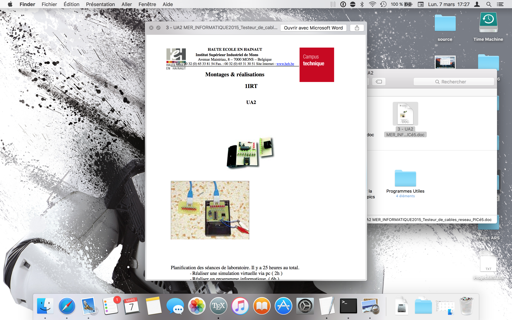
\includegraphics[width=\linewidth]
  {textures/images/mac/features/QuickLook.png}
  \caption{Quick Look}\label{fig: Quick Look}
	\endminipage\hfill \minipage{0.45\textwidth}
  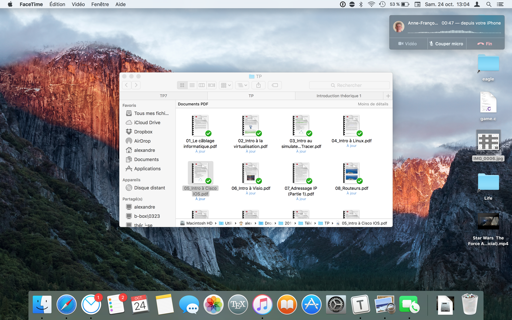
\includegraphics[width=\linewidth]{textures/images/mac/features/Phone.png}
  \caption{Téléphone}\label{fig:Telephone}
	\endminipage
\end{figure}

Pour terminer, Mac OS X ayant un noyau UNIX, l'utilisation du terminal y est à
peu près identique à celle sur Linux. \\
De plus, certains langages de programmation y sont déjà préinstallés comme Java,
Python, Ruby,…
